\section{Geom\-PQP2DRigid\-Multi  Class Reference}
\label{class_GeomPQP2DRigidMulti}\index{GeomPQP2DRigidMulti@{Geom\-PQP2DRigid\-Multi}}
A collection of 2D rigid bodies. 


{\tt \#include $<$geom\-PQP.h$>$}

Inheritance diagram for Geom\-PQP2DRigid\-Multi::\begin{figure}[H]
\begin{center}
\leavevmode
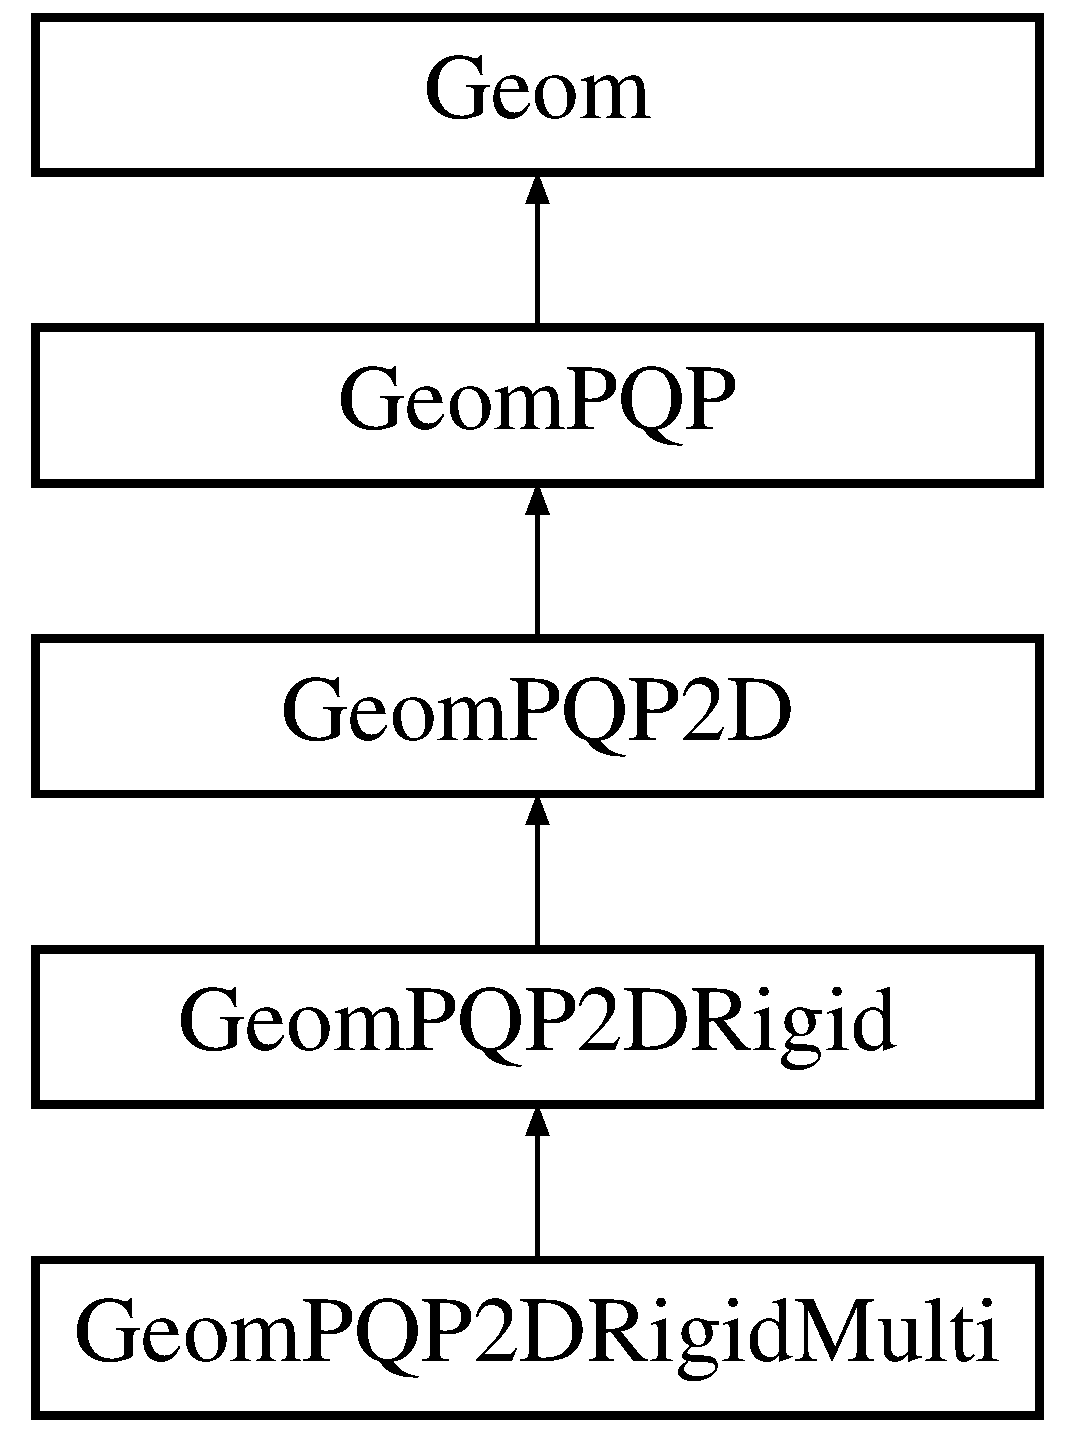
\includegraphics[height=5cm]{class_GeomPQP2DRigidMulti}
\end{center}
\end{figure}
\subsection*{Public Methods}
\begin{CompactItemize}
\item 
{\bf Geom\-PQP2DRigid\-Multi} (string path)
\item 
virtual {\bf $\sim$Geom\-PQP2DRigid\-Multi} ()
\item 
virtual bool {\bf Collision\-Free} (const {\bf MSLVector} \&q)
\begin{CompactList}\small\item\em Return true if the robot(s) and obstacles are not in collision.\item\end{CompactList}\item 
virtual double {\bf Distance\-Comp} (const {\bf MSLVector} \&q)
\begin{CompactList}\small\item\em Compute the distance of the closest point on the robot to the obstacle region.\item\end{CompactList}\item 
virtual void {\bf Load\-Robot} (string path)
\item 
void {\bf Set\-Transformation} (const {\bf MSLVector} \&q)
\end{CompactItemize}
\subsection*{Public Attributes}
\begin{CompactItemize}
\item 
bool {\bf Self\-Collision\-Check}
\end{CompactItemize}


\subsection{Detailed Description}
A collection of 2D rigid bodies.



\subsection{Constructor \& Destructor Documentation}
\index{GeomPQP2DRigidMulti@{Geom\-PQP2DRigid\-Multi}!GeomPQP2DRigidMulti@{GeomPQP2DRigidMulti}}
\index{GeomPQP2DRigidMulti@{GeomPQP2DRigidMulti}!GeomPQP2DRigidMulti@{Geom\-PQP2DRigid\-Multi}}
\subsubsection{\setlength{\rightskip}{0pt plus 5cm}Geom\-PQP2DRigid\-Multi::Geom\-PQP2DRigid\-Multi (string {\em path})}\label{class_GeomPQP2DRigidMulti_a0}


\index{GeomPQP2DRigidMulti@{Geom\-PQP2DRigid\-Multi}!~GeomPQP2DRigidMulti@{$\sim$GeomPQP2DRigidMulti}}
\index{~GeomPQP2DRigidMulti@{$\sim$GeomPQP2DRigidMulti}!GeomPQP2DRigidMulti@{Geom\-PQP2DRigid\-Multi}}
\subsubsection{\setlength{\rightskip}{0pt plus 5cm}Geom\-PQP2DRigid\-Multi::$\sim$Geom\-PQP2DRigid\-Multi ()\hspace{0.3cm}{\tt  [inline, virtual]}}\label{class_GeomPQP2DRigidMulti_a1}




\subsection{Member Function Documentation}
\index{GeomPQP2DRigidMulti@{Geom\-PQP2DRigid\-Multi}!CollisionFree@{CollisionFree}}
\index{CollisionFree@{CollisionFree}!GeomPQP2DRigidMulti@{Geom\-PQP2DRigid\-Multi}}
\subsubsection{\setlength{\rightskip}{0pt plus 5cm}virtual bool Geom\-PQP2DRigid\-Multi::Collision\-Free (const {\bf MSLVector} \& {\em q})\hspace{0.3cm}{\tt  [virtual]}}\label{class_GeomPQP2DRigidMulti_a2}


Return true if the robot(s) and obstacles are not in collision.



Reimplemented from {\bf Geom\-PQP2DRigid} {\rm (p.\,\pageref{class_GeomPQP2DRigid_a2})}.\index{GeomPQP2DRigidMulti@{Geom\-PQP2DRigid\-Multi}!DistanceComp@{DistanceComp}}
\index{DistanceComp@{DistanceComp}!GeomPQP2DRigidMulti@{Geom\-PQP2DRigid\-Multi}}
\subsubsection{\setlength{\rightskip}{0pt plus 5cm}virtual double Geom\-PQP2DRigid\-Multi::Distance\-Comp (const {\bf MSLVector} \& {\em q})\hspace{0.3cm}{\tt  [virtual]}}\label{class_GeomPQP2DRigidMulti_a3}


Compute the distance of the closest point on the robot to the obstacle region.



Reimplemented from {\bf Geom\-PQP2DRigid} {\rm (p.\,\pageref{class_GeomPQP2DRigid_a3})}.\index{GeomPQP2DRigidMulti@{Geom\-PQP2DRigid\-Multi}!LoadRobot@{LoadRobot}}
\index{LoadRobot@{LoadRobot}!GeomPQP2DRigidMulti@{Geom\-PQP2DRigid\-Multi}}
\subsubsection{\setlength{\rightskip}{0pt plus 5cm}virtual void Geom\-PQP2DRigid\-Multi::Load\-Robot (string {\em path})\hspace{0.3cm}{\tt  [virtual]}}\label{class_GeomPQP2DRigidMulti_a4}




Reimplemented from {\bf Geom\-PQP2D} {\rm (p.\,\pageref{class_GeomPQP2D_a3})}.\index{GeomPQP2DRigidMulti@{Geom\-PQP2DRigid\-Multi}!SetTransformation@{SetTransformation}}
\index{SetTransformation@{SetTransformation}!GeomPQP2DRigidMulti@{Geom\-PQP2DRigid\-Multi}}
\subsubsection{\setlength{\rightskip}{0pt plus 5cm}void Geom\-PQP2DRigid\-Multi::Set\-Transformation (const {\bf MSLVector} \& {\em q})}\label{class_GeomPQP2DRigidMulti_a5}




Reimplemented from {\bf Geom\-PQP2DRigid} {\rm (p.\,\pageref{class_GeomPQP2DRigid_a5})}.

\subsection{Member Data Documentation}
\index{GeomPQP2DRigidMulti@{Geom\-PQP2DRigid\-Multi}!SelfCollisionCheck@{SelfCollisionCheck}}
\index{SelfCollisionCheck@{SelfCollisionCheck}!GeomPQP2DRigidMulti@{Geom\-PQP2DRigid\-Multi}}
\subsubsection{\setlength{\rightskip}{0pt plus 5cm}bool Geom\-PQP2DRigid\-Multi::Self\-Collision\-Check}\label{class_GeomPQP2DRigidMulti_m0}




The documentation for this class was generated from the following file:\begin{CompactItemize}
\item 
{\bf geom\-PQP.h}\end{CompactItemize}
